\documentclass[12pt,a4paper]{report}
\setlength\textwidth{145mm}
 \setlength\topmargin{0mm}
 \setlength\headsep{0mm}
 \setlength\headheight{0mm}
 
% Přepneme na českou sazbu
\usepackage[czech]{babel}
\usepackage[IL2]{fontenc}
\usepackage{graphicx} 

%% Použité kódování znaků: obvykle latin2, cp1250 nebo utf8:
\usepackage[utf8]{inputenc}
\begin{document}

\chapter*{Hešování}
Ve všech následujících testech se používají klíče z univerza o velikosti $2^{64}$.

\section*{Náhodný testovací případ}
V tomto testu jsme vždy používali tabulky velikosti $2^{21}$ a veškeré měření jsou 
průměrována přes $20000$ vložení. Tabulky s lineárním přidáváním
byly testovány až do faktoru zaplnění $0.98$. Vkládání do kukaččí tabulky bylo přerušeno
pokud se alespoň $5$-krát za sebou nepovedl rehash.

\subsection*{Výběr vhodné konstanty $c$ pro tabulační hešování}
Jak ukazuje následující graf nejlépe vychází dělení klíče na 8 či 16 částí. 
Následující grafy ukazují čas na celé vložení prvku, nikoliv pouze hešování.
Nicméně, jelikož vkládáme náhodná data je vliv špatné heše resp. počet kroků při v kládání 
omezen a rozdíly v časech by měly reflektovat dobu výpočtu heše.

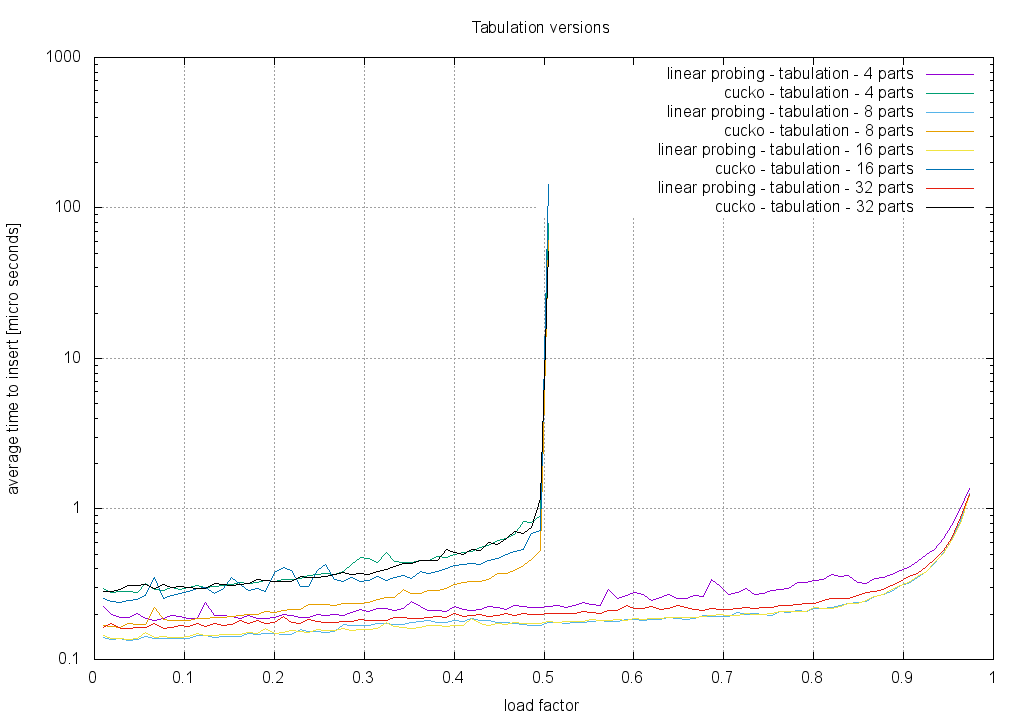
\includegraphics[width=\textwidth]{./tests/time_test/tabulation-hash-test.png}


\subsection*{Porovnání průměrné doby na vložení do tabulky}
Z grafu je vidět, že naivní a multiplikativní hešovací funkce potřebuje 
průměrně nejmenší dobu na insert. Je to způsobeno tím, že do tabulky vkládáme 
náhodná data. Proto doba reflektuje dobu výpočtu heše, která je pro tabulační heš nejsložitější.

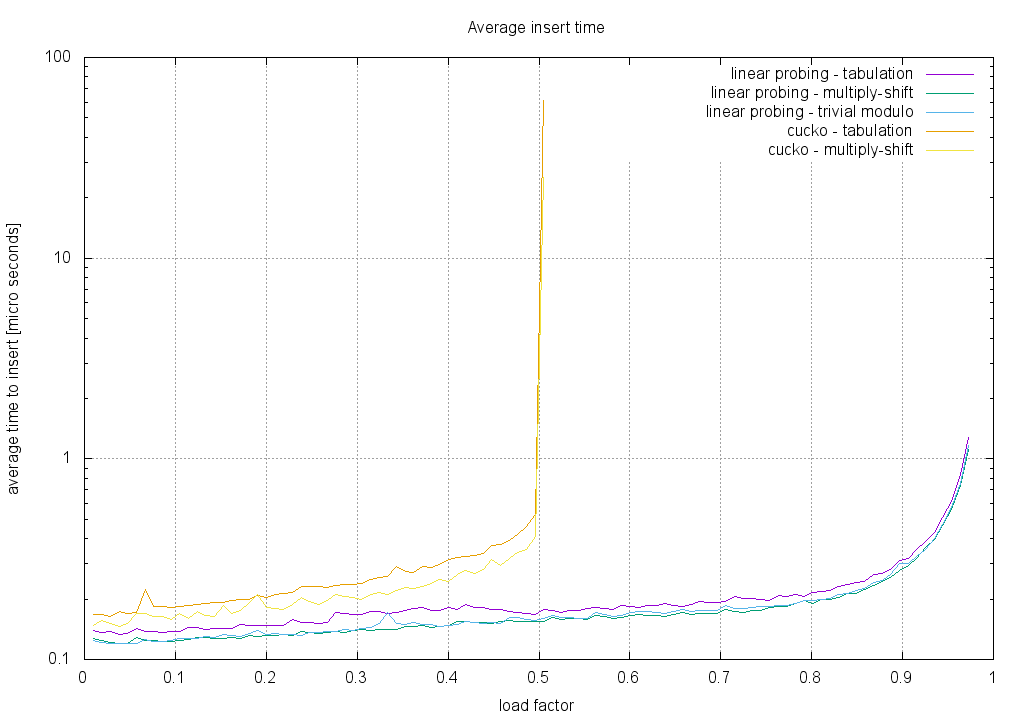
\includegraphics[width=\textwidth]{./tests/time_test/uniform-test8.png}

\subsection*{Porovnání průměrného počtu kroků na vložení do tabulky}

V následujícím grafu je vidět, že pokud vkládáme náhodná data, tak mezi použitými hešovacími funkcemi 
skutečně není rozdíl v kvalitě heše. Počty kroků jsou pro všechny typy heší srovnatelné a to v obou
typech tabulek. V obou grafech je také vidět, že pro kukaččí tabulku odpovídá teoretický faktor zaplnění $0.5$.

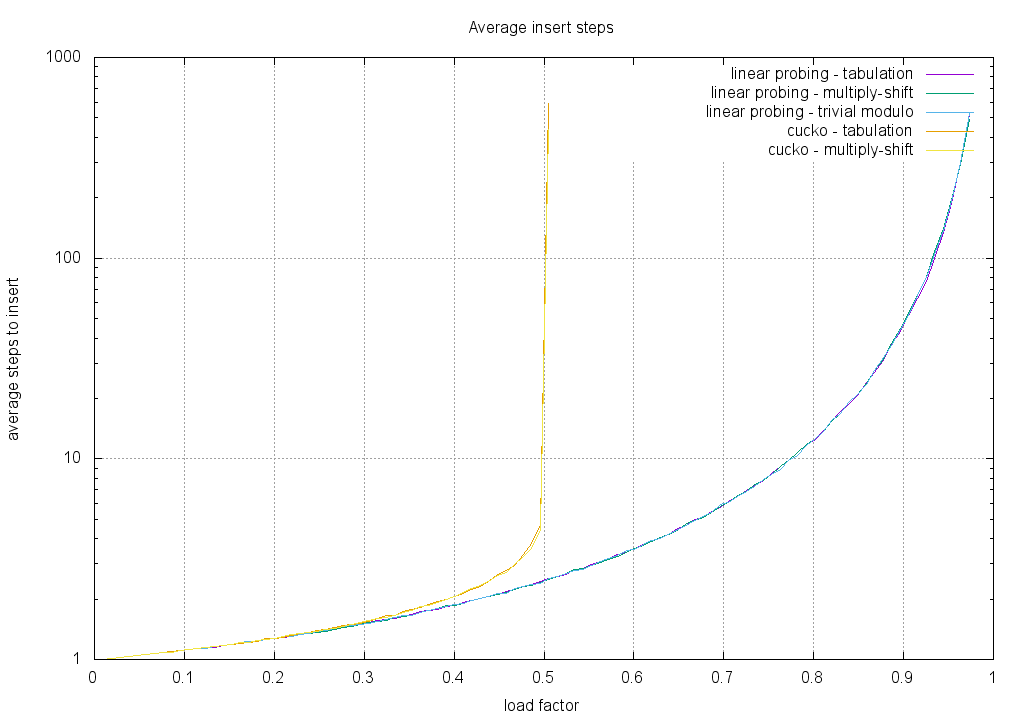
\includegraphics[width=\textwidth]{./tests/steps_test/uniform-test.png}

\section*{Sekvenční testovací případ}
V tomto případě byla použita tabelační hešovací funkce dělící klíč na 16 částí.
Zkoušeli jsme i dělení na 8 částí, které dopadlo obdobně. Pro první verzi jsme
prováděli testy pro větší tabulky až $2^{19}$, proto je zde uvádíme.

Bylo prováděno vždy $100000$ pokusů pro každou velikost tabulky, kde každý pokus 
je průměrný počet kroků na vložení pro faktor zaplnění v intervalu od $0.89$ do $0.91$.

\subsection*{Průměr a medián}
Z průměru a mediánu je výsledek ve prospěch multiplikativní hešovací funkce. 

Z rozdílu mezi průměrem a medianém je vidět, že pro tabluky přibližně od velikosti
$2^{14}$ jsou jednotlivé testy nevybalancované. Zdá se, že v některých pokusech
je u tabelační funkce dosaženo velmi malého počtu kroků. A naopak u multiplikativní
funkce v některých pokusech jsou počty kroků velmi velké.

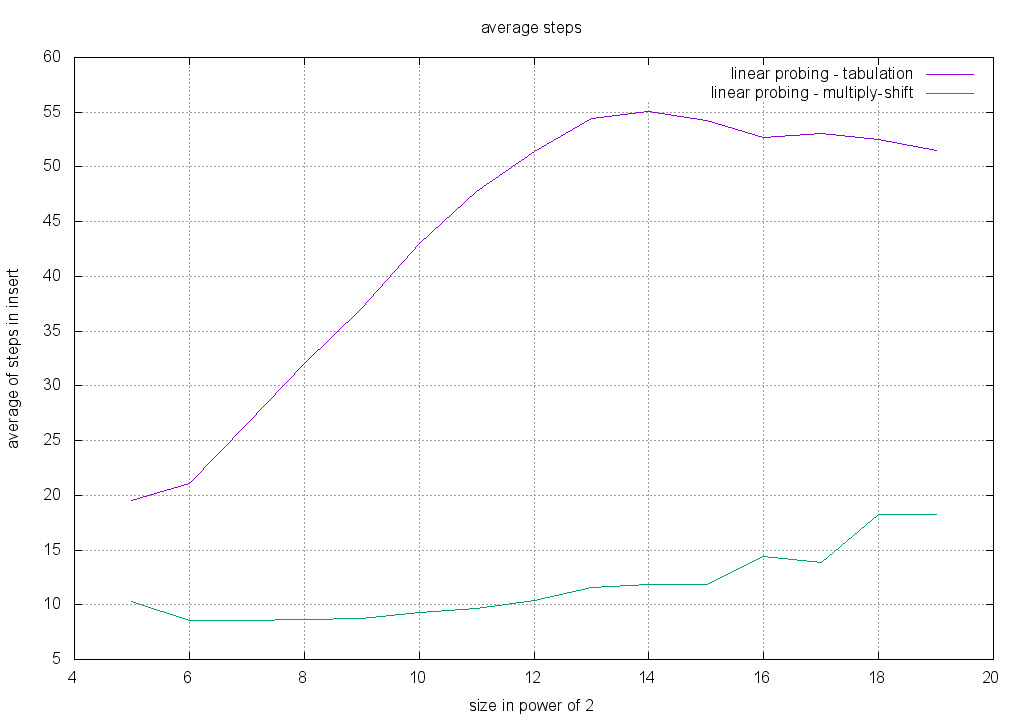
\includegraphics[width=\textwidth]{./tests/sequence_test/sequential-average-test.png}
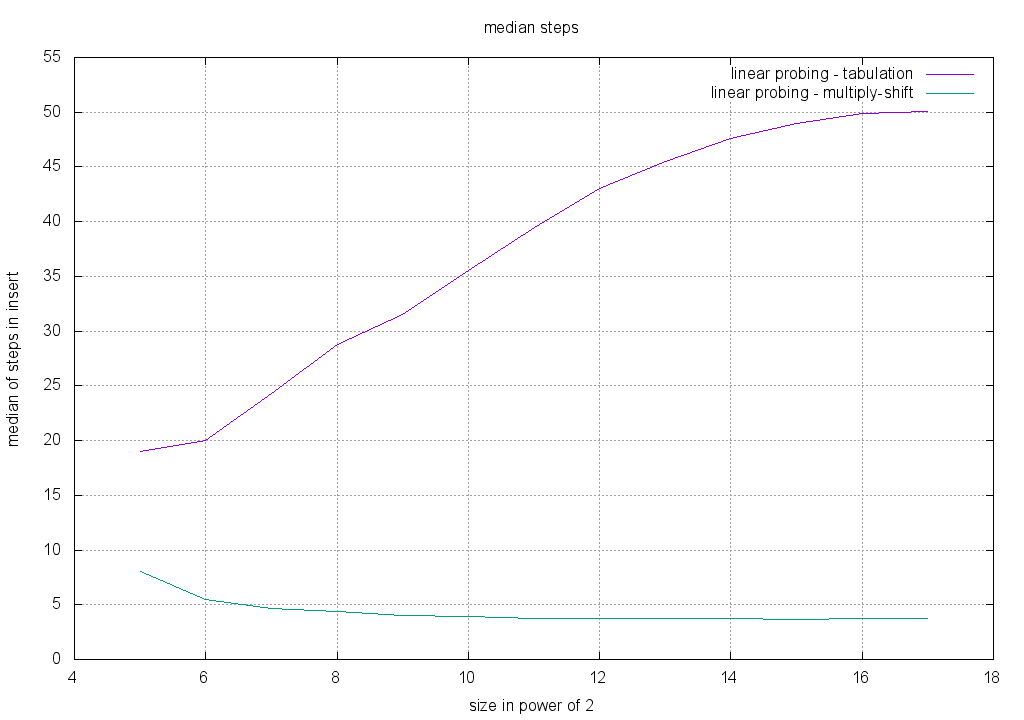
\includegraphics[width=\textwidth]{./tests/sequence_test/sequential-median-test.png}

\subsection*{Decil}
Z decilu je vidět, že $90 \%$ pokusů u multiplikativní funkce dává dobré výsldky.
Nárůst počtu kroků tedy je nejvýše v $10 \%$ případů.

Pro tabelační funkci dochází pro velké tabulky, ke snižování počtů špatných pokusů.

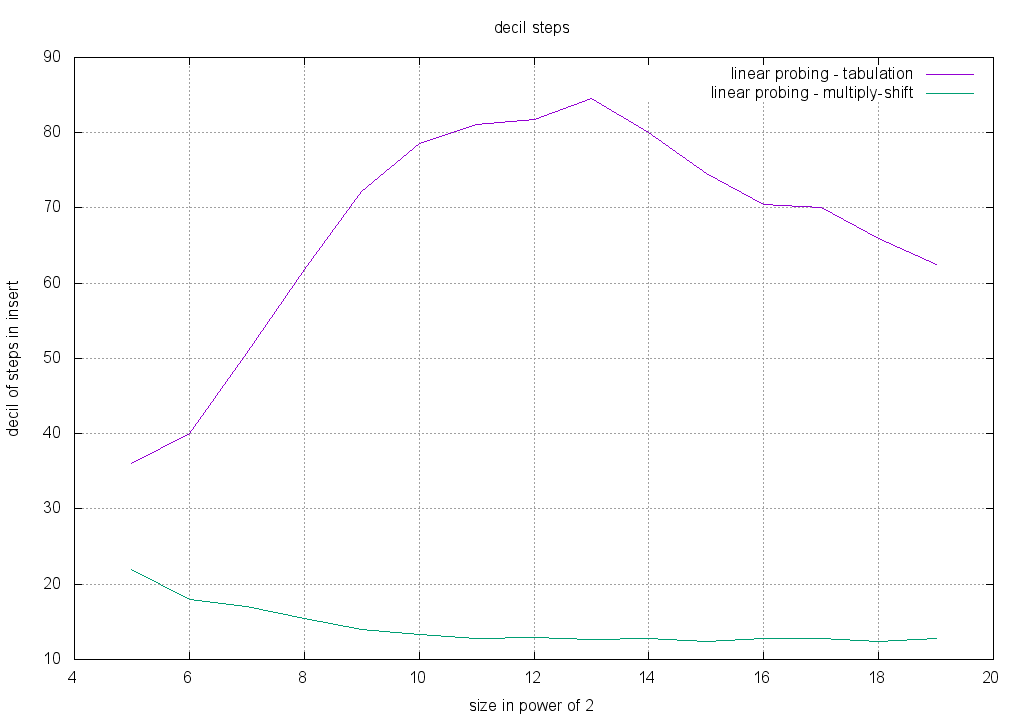
\includegraphics[width=\textwidth]{./tests/sequence_test/sequential-decil-test.png}


\subsection*{Maximum}
Zde se potvrzuje, že v případě multiplikativní funkce může dojít k hodně špatným výsledkům.
Naopak tabelační funkce dává  mnohem menší negativní extrémy.

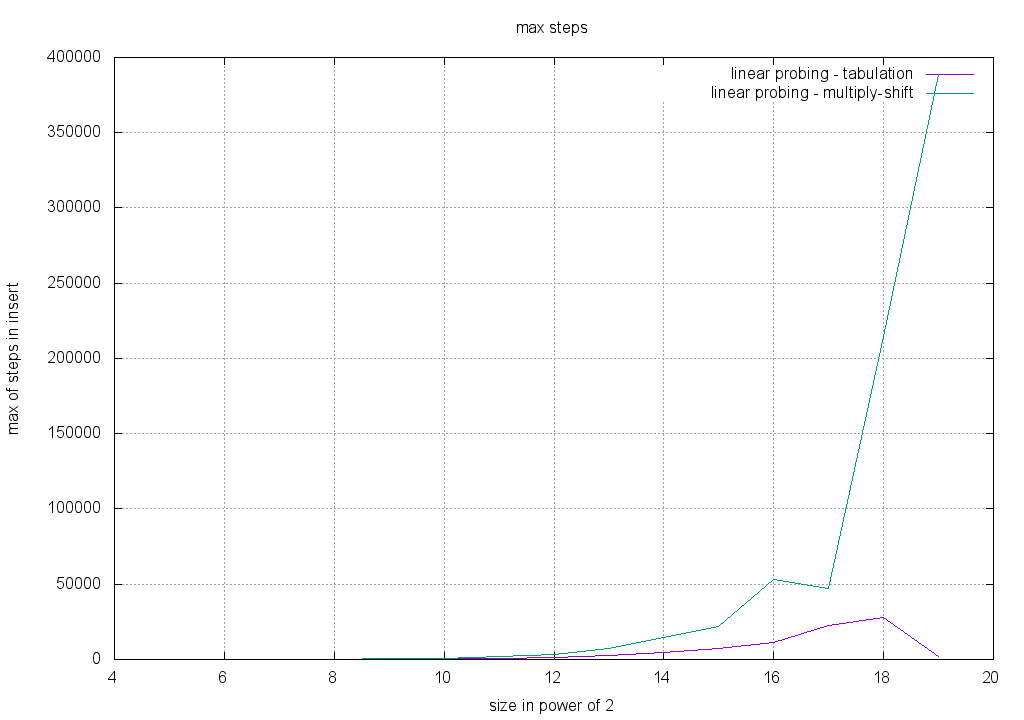
\includegraphics[width=\textwidth]{./tests/sequence_test/sequential-max-test.png}

\subsection*{Minimum}
Zde je situace opět opačná, multiplikativní funkce dokáže dávat mnohem lepší pozitivní 
hodnoty a to nezávisle na velikosti tabulky. Pro tabelační funkci se nejlepší hodnoty zhoršují 
s velikostí tabulky.

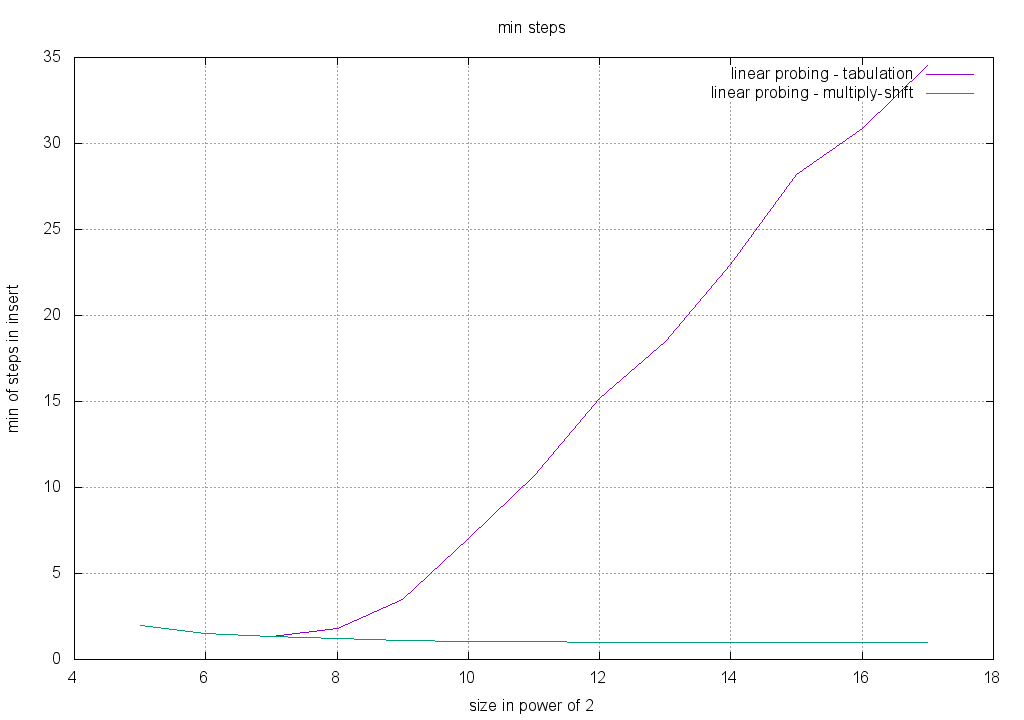
\includegraphics[width=\textwidth]{./tests/sequence_test/sequential-min-test.png}


\end{document}
